\documentclass[12]{article}

%Spell Check
\usepackage[british]{babel}

% Header & Footer
\usepackage{lipsum}
\usepackage{geometry}
\usepackage{fancyhdr}
\usepackage{charter}

% Bibliograhpy
\usepackage[super,numbers,sort&compress]{natbib}

%Image Software
\usepackage{graphicx}
\usepackage[space]{grffile}
\usepackage{float}

%Equation Software
\usepackage{bm}

\pagestyle{fancy}
\fancyhead{}
\fancyfoot{}
\fancyhead[R]{Page \thepage}
\renewcommand{\headrulewidth}{0.5pt}
\renewcommand{\footrulewidth}{0.5pt}

\begin{document}
\begin{titlepage}
\begin{center}
	
	\LARGE{\bf{Tobor Inc Automation Process}}\\
	[1cm]
	\large{J. R. Harper \\ QA Consulting \\ Project Supervisor: Roberto Fernandez}\\
	\large{Chris Lucas: Consultant Project Liason } \\
	[0.2cm]
	\line(1,0){400} \\
	
\end{center}


\end{titlepage}

\cleardoublepage

\tableofcontents

\thispagestyle{empty}
\pagenumbering{arabic}

\cleardoublepage

%First page

\section{Introduction}\label{sec:intro}

\setcounter{page}{1}

\subsection{Introduction}

Aims

\subsection{States}

There are several sattes and proggression points that ae wanted from this automation, starting with what the current siutation is and what is expected to happen.

\subsubsection{Current}

\begin{figure}[H]
	\centering
	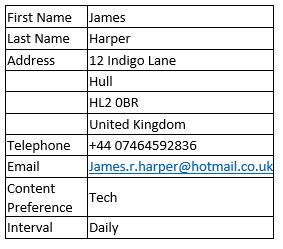
\includegraphics[height=3in]{C:/Users/james/Documents/Work/QA Consulting/Training Notes/Project (5 - 9)/Documentation/Images/Email Table}
	\caption[RegistrationTable]{Table used for registration}
	\label{fig:RegistrationTable}
\end{figure}

\subsubsection{Planned}

As was seen in figure \ref{fig:RegistrationTable} Tobor Inc. started out with using a HTML table sent through an email. This has now been adpapted for automation use with each box having an index of zero through to twenty, with the properties tables being zero, two, four etc... and the information being one, three, five etc... These tables can now be used as the standard format, as before, but with the robot calling the required index

\subsubsection{Benefits}

\subsubsection{Challenges}


\subsection{Example For Code Use}


\begin{equation}\label{eq:LL}
\bm{\dot{M}} = \bm{ \gamma M} \; x \; \bm{ H_{eff}} - \bm{ \lambda M} \; x \; \bm{  (M } \; x \; \bm{ H_{eff})}
\end{equation}

\begin{table}[H]
\centering
\begin{tabular}{l|l|l|l}
Capping Layer Parameter                      & Permalloy (80/20) & Nickel                    & Iron                       \\ \hline
Magnetic Saturation (kA/m)          & 800                  & 484 & 1730 \\
Exchange Constant (pJ/m)           &  13                 & 10.5                      & 21                         \\
Density (kkm/m3) &   8.74                & 8.90                      & 7.87                       \\
Electrical Conductivity (MS/m)     &       14.05            & 0.4                       & 10         \\
Anisotropy Constant (MOe) & 47 & 6 & 10 \\
               
\end{tabular}
\end{table}

\begin{table}[H]
\centering
\begin{tabular}{l|l|l}
Cap Metal & Density (kkg/m) & Electrical Conductivity (MS/m) \\ \hline
No Cap    & n/a             & n/a                        \\
Gold      & 19.3            & 41                         \\
Palladium & 11.9            & 10                         \\
Ruthenium & 12.2            & 14                         \\
Tantalum  & 16.65           & 7.7                        \\
Platinum  & 21.45           & 9.43                       \\
Nichrome  & 0.84            & 1                         
\end{tabular}
\end{table}


\cleardoublepage

\end{document}